\scanpage{22}
\deleted{\unsure{On|Un} \unsure{procède|procéde|procédé} par récurrence sur $\operatorname{card} K$,} \inserted{On note d'abord que} \deleted{pour prouver que} (si $\mbox{
% BEGIN C022-G01
% observed full-scan bbox (1007, 150, 1292, 379); origin/baseline (1010, 216).
% Local x=X-1010, y=Y-216; x=0.008cm, y=-0.008cm.
% Owns V=X setminus the indexed union, S01, the flat bracket and two descending equality strokes, and the inserted indexed intersection with S03.
\begin{tikzpicture}[baseline={(0,0)},x=0.008cm,y=-0.008cm,line cap=round,line join=round]
\path[use as bounding box] (-3,-66) rectangle (282,163);
\node[anchor=base west,inner sep=0,outer sep=0,font=\large] at (0,0) {$V=$};
\node[anchor=base west,inner sep=0,outer sep=0,font=\large] at (77,0) {$X\setminus$};
\node[anchor=base west,inner sep=0,outer sep=0,font=\large] at (148,-2) {$\bigcup_{\alpha\in K}$};
% Fixed-origin node for C022-S01: base-west at full (1211, 213), inner box xmin=-1, inner origin=(1212, 213).
\node[anchor=base west,inner sep=0,outer sep=0,font=\small] at (201,-3) {% BEGIN C022-S01
% full-scan origin/baseline (1212, 213); local x=X-1212, y=Y-213; x=0.008cm, y=-0.008cm.
% Owns one Sigma body, its short head, index \alpha, raised +, and the listed roof/bar/point only.
% Upper-run role: head/retrace or independent upper run unresolved.
\unsure{\mbox{\begin{tikzpicture}[baseline={(0,0)},x=0.008cm,y=-0.008cm,line cap=round,line join=round]
\path[use as bounding box] (-1,-58) rectangle (78,9);
\draw[line width=.55pt] (5,-29) -- (42,-27);
\draw[line width=.55pt] (4,-23) -- (37,-14) -- (5,-1) -- (43,0);
\draw[line width=.55pt] (23,-45) -- (45,-58) -- (62,-45);
\node[anchor=base west,inner sep=0,outer sep=0,font=\scriptsize] at (43,8) {$\alpha$};
\draw[line width=.55pt] (53,-28) -- (65,-28);
\draw[line width=.55pt] (59,-34) -- (59,-22);
\end{tikzpicture}}}
% END C022-S01
};
\draw[line width=.4pt] (71,39) -- (70,53) -- (74,57) -- (247,56) -- (254,52) -- (252,44);
\draw[line width=.55pt] (151,69) -- (152,83);
\draw[line width=.55pt] (161,70) -- (162,84);
\node[anchor=base west,inner sep=0,outer sep=0,font=\large] at (108,124) {$\bigcap_{\alpha\in K}$};
% Fixed-origin node for C022-S03: base-west at full (1164, 339), inner box xmin=-1, inner origin=(1165, 339).
\node[anchor=base west,inner sep=0,outer sep=0,font=\small] at (154,123) {% BEGIN C022-S03
% full-scan origin/baseline (1165, 339); local x=X-1165, y=Y-339; x=0.008cm, y=-0.008cm.
% Owns one Sigma body, its short head, index \alpha, raised -, and the listed roof/bar/point only.
% Upper-run role: head joins the angled body at its left end.
\mbox{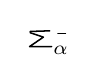
\begin{tikzpicture}[baseline={(0,0)},x=0.008cm,y=-0.008cm,line cap=round,line join=round]
\path[use as bounding box] (-1,-31) rectangle (72,12);
\draw[line width=.55pt] (3,-25) -- (34,-26);
\draw[line width=.55pt] (3,-23) -- (24,-16) -- (2,-1) -- (37,-1);
\node[anchor=base west,inner sep=0,outer sep=0,font=\scriptsize] at (40,11) {$\alpha$};
\draw[line width=.55pt] (47,-22) -- (59,-22);
\end{tikzpicture}}
% END C022-S03
};
\node[anchor=base west,inner sep=0,outer sep=0,font=\small,overlay] at (108,124) {$\phantom{\inserted{\bigcap_{\alpha\in K}\Sigma_\alpha^-}}$};
\end{tikzpicture}
% END C022-G01
}$, les $% BEGIN C022-S02
% full-scan origin/baseline (1448, 214); local x=X-1448, y=Y-214; x=0.008cm, y=-0.008cm.
% Owns one Sigma body, its short head, index \alpha, raised +, and the listed roof/bar/point only.
% Upper-run role: head/retrace or independent upper run unresolved.
\mbox{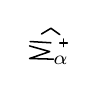
\begin{tikzpicture}[baseline={(0,0)},x=0.008cm,y=-0.008cm,line cap=round,line join=round]
\path[use as bounding box] (-1,-51) rectangle (74,9);
\draw[line width=.55pt] (3,-29) -- (36,-27);
\draw[line width=.55pt] (2,-22) -- (34,-13) -- (2,-2) -- (40,-1);
\draw[line width=.55pt] (21,-41) -- (36,-50) -- (50,-40);
\node[anchor=base west,inner sep=0,outer sep=0,font=\scriptsize] at (40,8) {$\alpha$};
\draw[line width=.55pt] (50,-27) -- (62,-27);
\draw[line width=.55pt] (56,-33) -- (56,-21);
\end{tikzpicture}}
% END C022-S02
$ ($\alpha\in K$\unsure{\mbox{
% BEGIN C022-G02
% observed full-scan bbox (1658, 207, 1679, 241); origin/baseline (1661, 237).
% Local x=X-1661, y=Y-237; x=0.008cm, y=-0.008cm.
% Owns the partial closing curve after K only; primary ) / blank interpretation remains qualified.
\begin{tikzpicture}[baseline={(0,0)},x=0.008cm,y=-0.008cm,line cap=round,line join=round]
\path[use as bounding box] (-3,-30) rectangle (18,4);
\draw[line width=.35pt] (1,-24) -- (8,-15) -- (16,2);
\node[anchor=base west,inner sep=0,outer sep=0,font=\small,overlay] at (0,0) {$\phantom{\unsure{)|}}$};
\end{tikzpicture}
% END C022-G02
}} étant \unsure{disjoints|disjointes})
\[
\mbox{
% BEGIN C022-G04
% observed full-scan bbox (390, 265, 1615, 485); origin/baseline (390, 340).
% Local x=X-390, y=Y-340; x=0.008cm, y=-0.008cm.
% Owns both conditions, S04 and S05, G03, the looped brace, trivial and its crossing arrow.
\begin{tikzpicture}[baseline={(0,0)},x=0.008cm,y=-0.008cm,line cap=round,line join=round]
\path[use as bounding box] (0,-75) rectangle (1225,145);
\node[anchor=base west,inner sep=0,outer sep=0,font=\large] at (200,0) {$\overline V\cap E_\alpha\ne\varnothing$};
\node[anchor=base west,inner sep=0,outer sep=0,font=\large] at (200,115) {$V\cap$};
% Fixed-origin node for C022-S04: base-west at full (681, 449), inner box xmin=-1, inner origin=(682, 449).
\node[anchor=base west,inner sep=0,outer sep=0,font=\small] at (291,109) {% BEGIN C022-S04
% full-scan origin/baseline (682, 449); local x=X-682, y=Y-449; x=0.008cm, y=-0.008cm.
% Owns one Sigma body, its short head, index \alpha, raised -, and the listed roof/bar/point only.
% Upper-run role: head/retrace or independent upper run unresolved.
\mbox{\begin{tikzpicture}[baseline={(0,0)},x=0.008cm,y=-0.008cm,line cap=round,line join=round]
\path[use as bounding box] (-1,-48) rectangle (100,14);
\draw[line width=.55pt] (4,-40) -- (45,-45);
\draw[line width=.55pt] (2,-33) -- (33,-25) -- (6,-3) -- (48,-2);
\node[anchor=base west,inner sep=0,outer sep=0,font=\scriptsize] at (51,13) {$\alpha$};
\draw[line width=.55pt] (70,-43) -- (82,-43);
\end{tikzpicture}}
% END C022-S04
};
% Fixed-origin node for C022-G03: base-west at full (794, 449), inner box xmin=-5, inner origin=(799, 449).
\node[anchor=base west,inner sep=0,outer sep=0,font=\small] at (404,109) {\unsure{\mbox{% BEGIN C022-G03
% observed full-scan bbox (794, 384, 922, 477); origin/baseline (799, 449).
% Local x=X-799, y=Y-449; x=0.008cm, y=-0.008cm.
% Owns the old relation and old empty-set shape, their cancelling strokes, and invisible annotation deleted neq/equals + empty-set.
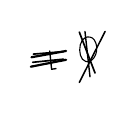
\begin{tikzpicture}[baseline={(0,0)},x=0.008cm,y=-0.008cm,line cap=round,line join=round]
\path[use as bounding box] (-5,-65) rectangle (123,28);
\draw[line width=.6pt] (4,-23) -- (52,-27);
\draw[line width=.6pt] (3,-10) -- (52,-15);
\draw[line width=.5pt] (30,-28) -- (33,1) -- (40,0);
\draw[line width=.8pt] (1,-18) -- (56,-28);
\draw[line width=.8pt] (0,-3) -- (56,-14);
\draw[line width=.4pt] (94,-50) .. controls (72,-55) and (72,-3) .. (95,-12) .. controls (111,-23) and (105,-49) .. (94,-50);
\draw[line width=.55pt] (77,22) -- (118,-59);
\draw[line width=.6pt] (77,-58) -- (102,7);
\draw[line width=.5pt] (86,-59) -- (94,13);
\node[anchor=base west,inner sep=0,outer sep=0,font=\small,overlay] at (0,0) {$\phantom{\deleted{\unsure{\ne|=}\varnothing}}$};
\end{tikzpicture}
% END C022-G03
}}};
\node[anchor=base west,inner sep=0,outer sep=0,font=\large] at (546,111) {$\ne\varnothing$};
\node[anchor=base west,inner sep=0,outer sep=0,font=\small] at (700,102) {alors que};
\node[anchor=base west,inner sep=0,outer sep=0,font=\large] at (950,100) {$V\cap$};
% Fixed-origin node for C022-S05: base-west at full (1410, 432), inner box xmin=-2, inner origin=(1412, 432).
\node[anchor=base west,inner sep=0,outer sep=0,font=\small] at (1020,92) {% BEGIN C022-S05
% full-scan origin/baseline (1412, 432); local x=X-1412, y=Y-432; x=0.008cm, y=-0.008cm.
% Owns one Sigma body, its short head, index \alpha, raised +, and the listed roof/bar/point only.
% Upper-run role: head/retrace or independent upper run unresolved.
\mbox{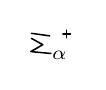
\begin{tikzpicture}[baseline={(0,0)},x=0.008cm,y=-0.008cm,line cap=round,line join=round]
\path[use as bounding box] (-2,-40) rectangle (78,15);
\draw[line width=.55pt] (4,-31) -- (33,-27);
\draw[line width=.55pt] (4,-23) -- (22,-13) -- (3,-2) -- (35,1);
\node[anchor=base west,inner sep=0,outer sep=0,font=\scriptsize] at (37,11) {$\alpha$};
\draw[line width=.55pt] (54,-30) -- (66,-30);
\draw[line width=.55pt] (60,-36) -- (60,-24);
\end{tikzpicture}}
% END C022-S05
};
\node[anchor=base west,inner sep=0,outer sep=0,font=\large] at (1108,100) {$=\varnothing$};
\draw[line width=.4pt] (158,-43) .. controls (167,-11) and (163,25) .. (156,43) .. controls (143,38) and (144,59) .. (153,50) .. controls (166,42) and (164,80) .. (165,114) .. controls (165,126) and (165,132) .. (169,137);
\node[anchor=base west,inner sep=0,outer sep=0,font=\scriptsize] at (24,111) {trivial};
\draw[line width=.3pt] (92,103) -- (191,94);
\draw[line width=.4pt] (184,90) -- (192,94) -- (184,98);
\end{tikzpicture}
% END C022-G04
}
\]
\par
De façon précise, je dis que
\figure{
% BEGIN C022-G05
% observed full-scan bbox (245, 630, 1667, 1935); origin/baseline (245, 630).
% Local x=X-245, y=Y-630; x=0.008cm, y=-0.008cm.
% Owns the main equality and its annotations, S06-S15, G06-G07, the cancelled proof and inserted égalité, all connected cancellation runs, the live Or sentence with both underlines, M01 and M02.
\begin{tikzpicture}[baseline={(0,0)},x=0.008cm,y=-0.008cm,line cap=round,line join=round]
\path[use as bounding box] (0,0) rectangle (1422,1305);
\node[anchor=base west,inner sep=0,outer sep=0,font=\large] at (365,95) {$\overline V\cap E_\alpha=$};
% Fixed-origin node for C022-S06: base-west at full (907, 718), inner box xmin=-2, inner origin=(909, 718).
\node[anchor=base west,inner sep=0,outer sep=0,font=\small] at (662,88) {% BEGIN C022-S06
% full-scan origin/baseline (909, 718); local x=X-909, y=Y-718; x=0.008cm, y=-0.008cm.
% Owns one Sigma body, its short head, index \alpha, raised -, and the listed roof/bar/point only.
% Upper-run role: head and angled body meet at the left end; outer closure rule is separate.
\mbox{\begin{tikzpicture}[baseline={(0,0)},x=0.008cm,y=-0.008cm,line cap=round,line join=round]
\path[use as bounding box] (-2,-75) rectangle (108,16);
\draw[line width=.55pt] (7,-50) -- (56,-49);
\draw[line width=.55pt] (6,-49) -- (35,-28) -- (4,-3) -- (57,-5);
\draw[line width=.55pt] (11,-68) -- (83,-70);
\node[anchor=base west,inner sep=0,outer sep=0,font=\scriptsize] at (60,12) {$\alpha$};
\draw[line width=.55pt] (82,-42) -- (94,-42);
\end{tikzpicture}}
% END C022-S06
};
\node[anchor=base west,inner sep=0,outer sep=0,font=\large] at (793,92) {$\cap E_\alpha$};
\node[anchor=base west,inner sep=0,outer sep=0,font=\small] at (1009,74) {(qui est donc $\ne\varnothing$)};
\draw[line width=.55pt] (442,121) -- (451,136);
\draw[line width=.55pt] (454,123) -- (462,142);
% Fixed-origin node for C022-A01: base-west at full (724, 798), inner box xmin=-3, inner origin=(727, 798).
\node[anchor=base west,inner sep=0,outer sep=0,font=\small] at (479,168) {\unsure{\mbox{% BEGIN C022-A01
% observed full-scan bbox (724, 741, 877, 812); origin/baseline (727, 798).
% Local x=X-727, y=Y-798; x=0.008cm, y=-0.008cm.
% Owns the complete lower-left annotation, live inserted primary and cancelled inserted alternative; adjoining two separator ticks remain in G05.
\begin{tikzpicture}[baseline={(0,0)},x=0.008cm,y=-0.008cm,line cap=round,line join=round]
\path[use as bounding box] (-3,-57) rectangle (150,14);
\node[anchor=base west,inner sep=0,outer sep=0,font=\small] at (0,0) {$\overline V\cap$};
% Fixed-origin node for C022-S07: base-west at full (802, 788), inner box xmin=-1, inner origin=(803, 788).
\node[anchor=base west,inner sep=0,outer sep=0,font=\small] at (75,-10) {% BEGIN C022-S07
% full-scan origin/baseline (803, 788); local x=X-803, y=Y-788; x=0.008cm, y=-0.008cm.
% Owns one Sigma body, its short head, index \alpha, raised +, and the listed roof/bar/point only.
% Upper-run role: head/retrace or independent upper run unresolved.
\mbox{\begin{tikzpicture}[baseline={(0,0)},x=0.008cm,y=-0.008cm,line cap=round,line join=round]
\path[use as bounding box] (-1,-47) rectangle (71,18);
\draw[line width=.55pt] (4,-22) -- (33,-26);
\draw[line width=.55pt] (5,-18) -- (27,-11) -- (4,2) -- (37,0);
\draw[line width=.55pt] (14,-32) -- (30,-43) -- (45,-33);
\node[anchor=base west,inner sep=0,outer sep=0,font=\scriptsize] at (38,14) {$\alpha$};
\draw[line width=.55pt] (48,-20) -- (60,-20);
\draw[line width=.55pt] (54,-26) -- (54,-14);
\end{tikzpicture}}
% END C022-S07
};
\node[anchor=base west,inner sep=0,outer sep=0,font=\small,overlay] at (0,0) {$\phantom{\unsure{\inserted{\overline V\cap\widehat\Sigma_\alpha^+}|\deleted{\inserted{\overline V\cap\widehat\Sigma_\alpha^+}}}}$};
\end{tikzpicture}
% END C022-A01
}}};
% Fixed-origin node for C022-G06: base-west at full (1007, 750), inner box xmin=-1, inner origin=(1008, 750).
\node[anchor=base west,inner sep=0,outer sep=0,font=\small] at (762,120) {\unsure{\mbox{% BEGIN C022-G06
% observed full-scan bbox (1007, 734, 1074, 757); origin/baseline (1008, 750).
% Local x=X-1008, y=Y-750; x=0.008cm, y=-0.008cm.
% Owns one shared horizontal and three short oblique ticks; vertical deleted equals / equals / implication candidates, no second closure rule.

\begin{tikzpicture}[baseline={(0,0)},x=0.008cm,y=-0.008cm,line cap=round,line join=round]
\path[use as bounding box] (-1,-16) rectangle (66,7);
\draw[line width=.55pt] (2,-1) -- (60,0);
\draw[line width=.45pt] (9,2) -- (17,-6);
\draw[line width=.55pt] (46,-11) -- (52,-1);
\draw[line width=.55pt] (56,-11) -- (60,0);
\node[anchor=base west,inner sep=0,outer sep=0,font=\small,overlay] at (0,0) {$\phantom{\rotatebox{90}{$\unsure{\deleted{=}|=|\Rightarrow}$}}$};
\end{tikzpicture}
% END C022-G06
}}};
% Fixed-origin node for C022-A02: base-west at full (998, 786), inner box xmin=-2, inner origin=(1000, 786).
\node[anchor=base west,inner sep=0,outer sep=0,font=\small] at (753,156) {\unsure{\mbox{% BEGIN C022-A02
% observed full-scan bbox (998, 725, 1185, 801); origin/baseline (1000, 786).
% Local x=X-1000, y=Y-786; x=0.008cm, y=-0.008cm.
% Owns the complete lower-right formula: live inserted primary and deleted inserted alternative; shared upper run remains owned by G06.
\begin{tikzpicture}[baseline={(0,0)},x=0.008cm,y=-0.008cm,line cap=round,line join=round]
\path[use as bounding box] (-2,-61) rectangle (185,15);
% Fixed-origin node for C022-S08: base-west at full (998, 786), inner box xmin=-2, inner origin=(1000, 786).
\node[anchor=base west,inner sep=0,outer sep=0,font=\small] at (-2,0) {% BEGIN C022-S08
% full-scan origin/baseline (1000, 786); local x=X-1000, y=Y-786; x=0.008cm, y=-0.008cm.
% Owns one Sigma body, its short head, index \alpha, raised -, and the listed roof/bar/point only.
% Upper-run role: head/retrace or independent upper run unresolved.
\mbox{\begin{tikzpicture}[baseline={(0,0)},x=0.008cm,y=-0.008cm,line cap=round,line join=round]
\path[use as bounding box] (-2,-49) rectangle (80,9);
\draw[line width=.55pt] (5,-22) -- (37,-24);
\draw[line width=.55pt] (4,-16) -- (34,-10) -- (4,-1) -- (38,-2);
% Shared visible rule owned once by C022-G04 connector horizontal, (1009,749) to (1068,749).
\node[anchor=base west,inner sep=0,outer sep=0,font=\scriptsize] at (42,6) {$\alpha$};
\draw[line width=.55pt] (56,-19) -- (68,-19);
\end{tikzpicture}}
% END C022-S08
};
\node[anchor=base west,inner sep=0,outer sep=0,font=\small] at (89,-2) {$\cap$};
% Fixed-origin node for C022-S09: base-west at full (1119, 775), inner box xmin=-1, inner origin=(1120, 775).
\node[anchor=base west,inner sep=0,outer sep=0,font=\small] at (119,-11) {% BEGIN C022-S09
% full-scan origin/baseline (1120, 775); local x=X-1120, y=Y-775; x=0.008cm, y=-0.008cm.
% Owns one Sigma body, its short head, index \alpha, raised +, and the listed roof/bar/point only.
% Upper-run role: head/retrace or independent upper run unresolved.
\mbox{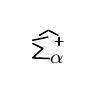
\begin{tikzpicture}[baseline={(0,0)},x=0.008cm,y=-0.008cm,line cap=round,line join=round]
\path[use as bounding box] (-1,-49) rectangle (63,12);
\draw[line width=.55pt] (7,-29) -- (31,-34);
\draw[line width=.55pt] (7,-24) -- (23,-16) -- (7,-1) -- (34,0);
\draw[line width=.55pt] (18,-37) -- (32,-45) -- (47,-37);
\node[anchor=base west,inner sep=0,outer sep=0,font=\scriptsize] at (34,8) {$\alpha$};
\draw[line width=.55pt] (43,-27) -- (55,-27);
\draw[line width=.55pt] (49,-33) -- (49,-21);
\end{tikzpicture}}
% END C022-S09
};
\node[anchor=base west,inner sep=0,outer sep=0,font=\small,overlay] at (0,0) {$\phantom{\unsure{\inserted{\overline{\Sigma_\alpha^-}\cap\widehat\Sigma_\alpha^+}|\deleted{\inserted{\overline{\Sigma_\alpha^-}\cap\widehat\Sigma_\alpha^+}}}}$};
\end{tikzpicture}
% END C022-A02
}}};
\node[anchor=base west,inner sep=0,outer sep=0,font=\small] at (15,216) {\rlap{Comme}\phantom{\deleted{Comme}}};
\node[anchor=base west,inner sep=0,outer sep=0,font=\small] at (380,216) {\rlap{$V\subset$}\phantom{\deleted{$V\subset$}}};
% Fixed-origin node for C022-S10: base-west at full (740, 844), inner box xmin=-1, inner origin=(741, 844).
\node[anchor=base west,inner sep=0,outer sep=0,font=\small] at (495,214) {% BEGIN C022-S10
% full-scan origin/baseline (741, 844); local x=X-741, y=Y-844; x=0.008cm, y=-0.008cm.
% Owns one Sigma body, its short head, index \alpha, raised -, and the listed roof/bar/point only.
% Upper-run role: upper head lies immediately below the crossing frame; exact joining is crowded.
\mbox{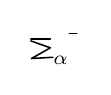
\begin{tikzpicture}[baseline={(0,0)},x=0.008cm,y=-0.008cm,line cap=round,line join=round]
\path[use as bounding box] (-1,-50) rectangle (86,12);
\draw[line width=.55pt] (4,-32) -- (35,-32);
\draw[line width=.55pt] (4,-29) -- (35,-18) -- (5,-1) -- (39,-3);
\node[anchor=base west,inner sep=0,outer sep=0,font=\scriptsize] at (40,9) {$\alpha$};
\draw[line width=.55pt] (65,-41) -- (77,-41);
\node[overlay,anchor=base west,inner sep=0,outer sep=0] at (0,0) {$\phantom{\deleted{\Sigma_{\alpha}^{-}}}$};
\end{tikzpicture}}
% END C022-S10
};
\node[anchor=base west,inner sep=0,outer sep=0,font=\small] at (630,218) {\rlap{, on a}\phantom{\deleted{, on a}}};
\node[anchor=base west,inner sep=0,outer sep=0,font=\small] at (928,216) {\rlap{$V\cap E_\alpha\subset$}\phantom{\deleted{$V\cap E_\alpha\subset$}}};
% Fixed-origin node for C022-S11: base-west at full (1400, 826), inner box xmin=-2, inner origin=(1402, 826).
\node[anchor=base west,inner sep=0,outer sep=0,font=\small] at (1155,196) {% BEGIN C022-S11
% full-scan origin/baseline (1402, 826); local x=X-1402, y=Y-826; x=0.008cm, y=-0.008cm.
% Owns one Sigma body, its short head, index \alpha, raised -, and the listed roof/bar/point only.
% Upper-run role: head/retrace or independent upper run unresolved.
\unsure{\mbox{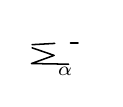
\begin{tikzpicture}[baseline={(0,0)},x=0.008cm,y=-0.008cm,line cap=round,line join=round]
\path[use as bounding box] (-2,-60) rectangle (105,21);
\draw[line width=.55pt] (5,-33) -- (41,-35);
\draw[line width=.55pt] (5,-28) -- (40,-16) -- (4,-3) -- (63,-2);
% Shared visible rule owned once by C022-G05 top frame, with dark local run (1410,774) to (1495,771).
\node[anchor=base west,inner sep=0,outer sep=0,font=\scriptsize] at (46,16) {$\alpha$};
\draw[line width=.55pt] (66,-36) -- (78,-36);
\node[overlay,anchor=base west,inner sep=0,outer sep=0] at (0,0) {$\phantom{\deleted{\overline{\Sigma_{\alpha}^{-}}}}$};
\end{tikzpicture}}}
% END C022-S11
};
\node[anchor=base west,inner sep=0,outer sep=0,font=\small] at (1275,214) {\rlap{$\cap E_\alpha$,}\phantom{\deleted{$\cap E_\alpha$,}}};
\node[anchor=base west,inner sep=0,outer sep=0,font=\small] at (27,346) {\rlap{prouvons}\phantom{\deleted{prouvons}}};
\node[anchor=base west,inner sep=0,outer sep=0,font=\small] at (330,327) {\rlap{l'inclusion inverse}\phantom{\deleted{l'inclusion inverse}}};
% Fixed-origin node for C022-S12: base-west at full (567, 1086), inner box xmin=-1, inner origin=(568, 1086).
\node[anchor=base west,inner sep=0,outer sep=0,font=\small] at (322,456) {% BEGIN C022-S12
% full-scan origin/baseline (568, 1086); local x=X-568, y=Y-1086; x=0.008cm, y=-0.008cm.
% Owns one Sigma body, its short head, index \alpha, raised -, and the listed roof/bar/point only.
% Upper-run role: head and body meet at the upper left; closure rule is separate.
\mbox{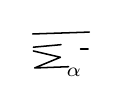
\begin{tikzpicture}[baseline={(0,0)},x=0.008cm,y=-0.008cm,line cap=round,line join=round]
\path[use as bounding box] (-1,-65) rectangle (111,15);
\draw[line width=.55pt] (8,-34) -- (52,-38);
\draw[line width=.55pt] (8,-28) -- (51,-18) -- (10,-1) -- (64,-3);
\draw[line width=.55pt] (7,-55) -- (97,-58);
\node[anchor=base west,inner sep=0,outer sep=0,font=\scriptsize] at (61,12) {$\alpha$};
\draw[line width=.55pt] (83,-31) -- (95,-31);
\node[overlay,anchor=base west,inner sep=0,outer sep=0] at (0,0) {$\phantom{\deleted{\overline{\Sigma_{\alpha}^{-}}}}$};
\end{tikzpicture}}
% END C022-S12
};
\node[anchor=base west,inner sep=0,outer sep=0,font=\small] at (432,451) {\rlap{$\cap E_\alpha\subset\overline V\cap E_\alpha$}\phantom{\deleted{$\cap E_\alpha\subset\overline V\cap E_\alpha$}}};
\node[anchor=base west,inner sep=0,outer sep=0,font=\small] at (41,578) {\rlap{Soit}\phantom{\deleted{Soit}}};
\node[anchor=base west,inner sep=0,outer sep=0,font=\small] at (236,574) {\rlap{$x\in$}\phantom{\deleted{$x\in$}}};
% Fixed-origin node for C022-S13: base-west at full (591, 1194), inner box xmin=-2, inner origin=(593, 1194).
\node[anchor=base west,inner sep=0,outer sep=0,font=\small] at (346,564) {% BEGIN C022-S13
% full-scan origin/baseline (593, 1194); local x=X-593, y=Y-1194; x=0.008cm, y=-0.008cm.
% Owns one Sigma body, its short head, index \alpha, raised -, and the listed roof/bar/point only.
% Upper-run role: head/retrace or independent upper run unresolved.
\mbox{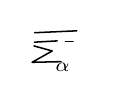
\begin{tikzpicture}[baseline={(0,0)},x=0.008cm,y=-0.008cm,line cap=round,line join=round]
\path[use as bounding box] (-2,-57) rectangle (88,19);
\draw[line width=.55pt] (9,-34) -- (45,-36);
\draw[line width=.55pt] (8,-28) -- (37,-20) -- (5,-2) -- (51,-3);
\draw[line width=.55pt] (9,-49) -- (76,-52);
\node[anchor=base west,inner sep=0,outer sep=0,font=\scriptsize] at (42,13) {$\alpha$};
\draw[line width=.55pt] (58,-35) -- (70,-35);
\node[overlay,anchor=base west,inner sep=0,outer sep=0] at (0,0) {$\phantom{\deleted{\overline{\Sigma_{\alpha}^{-}}}}$};
\end{tikzpicture}}
% END C022-S13
};
\node[anchor=base west,inner sep=0,outer sep=0,font=\small] at (427,574) {\rlap{$\cap E_\alpha$,}\phantom{\deleted{$\cap E_\alpha$,}}};
\node[anchor=base west,inner sep=0,outer sep=0,font=\small] at (622,567) {\rlap{prouvons}\phantom{\deleted{prouvons}}};
\node[anchor=base west,inner sep=0,outer sep=0,font=\small] at (925,561) {\rlap{$x\in\overline V\cap E_\alpha$ i.e.}\phantom{\deleted{$x\in\overline V\cap E_\alpha$ i.e.}}};
\node[anchor=base west,inner sep=0,outer sep=0,font=\small] at (10,679) {\rlap{$x\in\overline V$,}\phantom{\deleted{$x\in\overline V$,}}};
\node[anchor=base west,inner sep=0,outer sep=0,font=\small] at (254,669) {\rlap{soit}\phantom{\deleted{soit}}};
\node[anchor=base west,inner sep=0,outer sep=0,font=\small] at (415,662) {\rlap{$W$ un voisinage de $x$,}\phantom{\deleted{$W$ un voisinage de $x$,}}};
\node[anchor=base west,inner sep=0,outer sep=0,font=\small] at (1007,651) {\rlap{montrons qu'il}\phantom{\deleted{montrons qu'il}}};
\node[anchor=base west,inner sep=0,outer sep=0,font=\small] at (26,773) {\rlap{rencontre}\phantom{\deleted{rencontre}}};
\node[anchor=base west,inner sep=0,outer sep=0,font=\small] at (456,742) {\rlap{Or}\phantom{\deleted{Or}}};
\node[anchor=base west,inner sep=0,outer sep=0,font=\small] at (574,744) {\rlap{\unsure{on}}\phantom{\deleted{\unsure{on}}}};
\node[anchor=base west,inner sep=0,outer sep=0,font=\small] at (705,741) {\rlap{peut considérer cette}\phantom{\deleted{peut considérer cette}}};
\node[anchor=base west,inner sep=0,outer sep=0,font=\small] at (33,876) {\rlap{formule}\phantom{\deleted{formule}}};
\node[anchor=base west,inner sep=0,outer sep=0,font=\small] at (87,834) {\rlap{\inserted{égalité}}\phantom{\deleted{\inserted{égalité}}}};
\node[anchor=base west,inner sep=0,outer sep=0,font=\small] at (319,855) {\rlap{comme}\phantom{\deleted{comme}}};
\node[anchor=base west,inner sep=0,outer sep=0,font=\small] at (639,850) {\rlap{égalité dans}\phantom{\deleted{égalité dans}}};
\node[anchor=base west,inner sep=0,outer sep=0,font=\small] at (67,965) {\rlap{l'espace}\phantom{\deleted{l'espace}}};
% Fixed-origin node for C022-G07: base-west at full (572, 1626), inner box xmin=-4, inner origin=(576, 1626).
\node[anchor=base west,inner sep=0,outer sep=0,font=\small] at (327,996) {\unsure{\mbox{% BEGIN C022-G07
% observed full-scan bbox (572, 1558, 640, 1636); origin/baseline (576, 1626).
% Local x=X-576, y=Y-1626; x=0.008cm, y=-0.008cm.
% Owns the old cancelled variable, all visible crossing/foot strokes; primary Y with Z and H X alternatives.
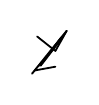
\begin{tikzpicture}[baseline={(0,0)},x=0.008cm,y=-0.008cm,line cap=round,line join=round]
\path[use as bounding box] (-4,-68) rectangle (64,10);
\draw[line width=.65pt] (11,-54) -- (40,-31) -- (58,-63);
\draw[line width=.7pt] (58,-63) -- (3,5);
\draw[line width=.65pt] (7,0) -- (40,-6);
\draw[line width=1.0pt] (16,-8) -- (50,-52);
\node[anchor=base west,inner sep=0,outer sep=0,font=\small,overlay] at (0,0) {$\phantom{\deleted{\unsure{Y|Z|X}}}$};
\end{tikzpicture}
% END C022-G07
}}};
\node[anchor=base west,inner sep=0,outer sep=0,font=\small] at (395,988) {\rlap{$=$}\phantom{\deleted{$=$}}};
% Fixed-origin node for C022-S14: base-west at full (716, 1617), inner box xmin=-2, inner origin=(718, 1617).
\node[anchor=base west,inner sep=0,outer sep=0,font=\small] at (471,987) {% BEGIN C022-S14
% full-scan origin/baseline (718, 1617); local x=X-718, y=Y-1617; x=0.008cm, y=-0.008cm.
% Owns one Sigma body, its short head, index \alpha, raised -, and the listed roof/bar/point only.
% Upper-run role: head/retrace or independent upper run unresolved.
\mbox{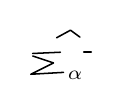
\begin{tikzpicture}[baseline={(0,0)},x=0.008cm,y=-0.008cm,line cap=round,line join=round]
\path[use as bounding box] (-2,-75) rectangle (114,8);
\draw[line width=.55pt] (6,-34) -- (50,-36);
\draw[line width=.55pt] (6,-30) -- (39,-19) -- (3,-1) -- (55,-4);
\draw[line width=.55pt] (44,-59) -- (66,-71) -- (81,-60);
\node[anchor=base west,inner sep=0,outer sep=0,font=\scriptsize] at (62,7) {$\alpha$};
\draw[line width=.55pt] (87,-36) -- (99,-36);
\node[overlay,anchor=base west,inner sep=0,outer sep=0] at (0,0) {$\phantom{\deleted{\widehat{\Sigma_{\alpha}^{-}}}}$};
\end{tikzpicture}}
% END C022-S14
};
\node[anchor=base west,inner sep=0,outer sep=0,font=\small] at (605,987) {\rlap{$=$}\phantom{\deleted{$=$}}};
% Fixed-origin node for C022-S15: base-west at full (892, 1615), inner box xmin=-3, inner origin=(895, 1615).
\node[anchor=base west,inner sep=0,outer sep=0,font=\small] at (647,985) {% BEGIN C022-S15
% full-scan origin/baseline (895, 1615); local x=X-895, y=Y-1615; x=0.008cm, y=-0.008cm.
% Owns one Sigma body, its short head, index \alpha, raised -, and the listed roof/bar/point only.
% Upper-run role: head/retrace or independent upper run unresolved.
\mbox{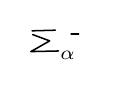
\begin{tikzpicture}[baseline={(0,0)},x=0.008cm,y=-0.008cm,line cap=round,line join=round]
\path[use as bounding box] (-3,-38) rectangle (90,13);
\draw[line width=.55pt] (4,-33) -- (41,-34);
\draw[line width=.55pt] (5,-27) -- (32,-17) -- (2,0) -- (46,-1);
\node[anchor=base west,inner sep=0,outer sep=0,font=\scriptsize] at (49,12) {$\alpha$};
\draw[line width=.55pt] (66,-28) -- (78,-28);
\node[overlay,anchor=base west,inner sep=0,outer sep=0] at (0,0) {$\phantom{\deleted{\Sigma_{\alpha}^{-}}}$};
\end{tikzpicture}}
% END C022-S15
};
\node[anchor=base west,inner sep=0,outer sep=0,font=\small] at (754,988) {\rlap{$\cup E_\alpha$}\phantom{\deleted{$\cup E_\alpha$}}};
\node[anchor=base west,inner sep=0,outer sep=0,font=\small] at (62,1100) {\rlap{dans lequel on a deux parties fermées}\phantom{\deleted{dans lequel on a deux parties fermées}}};
\node[anchor=base west,inner sep=0,outer sep=0,font=\small] at (61,1212) {\rlap{disjointes}\phantom{\deleted{disjointes}}};
\node[anchor=base west,inner sep=0,outer sep=0,font=\small] at (473,1166) {Or dans $X$ on a les deux};
\node[anchor=base west,inner sep=0,outer sep=0,font=\small] at (64,1283) {parties};
\node[anchor=base west,inner sep=0,outer sep=0,font=\small] at (335,1278) {\uline{fermées}};
\node[anchor=base west,inner sep=0,outer sep=0,font=\small] at (595,1276) {\uline{disjointes}};
% BEGIN C022-G05-PATHS
\draw[line width=.4pt] (1324,146) .. controls (1194,136) and (812,153) .. (476,170) .. controls (305,184) and (161,206) .. (29,205);
\draw[line width=.4pt] (29,205) .. controls (45,278) and (54,417) .. (54,554) .. controls (69,616) and (64,686) .. (40,770);
\draw[line width=.4pt] (40,770) .. controls (144,780) and (302,757) .. (394,751) .. controls (373,710) and (374,663) .. (418,658) .. controls (650,661) and (884,660) .. (1076,656);
\draw[line width=.4pt] (40,770) .. controls (42,817) and (31,861) .. (47,876) .. controls (140,870) and (368,846) .. (664,840) .. controls (896,826) and (1085,857) .. (1189,824) .. controls (1260,803) and (1267,722) .. (1355,690);
\draw[line width=.4pt] (68,875) .. controls (65,916) and (63,951) .. (68,972) .. controls (87,1011) and (236,981) .. (358,969) .. controls (537,947) and (741,985) .. (872,978) .. controls (958,974) and (1039,947) .. (1100,911);
\draw[line width=.4pt] (63,1098) .. controls (294,1084) and (534,1063) .. (712,1074) .. controls (897,1087) and (1092,1075) .. (1272,1081);
\draw[line width=.4pt] (63,1098) .. controls (58,1136) and (40,1185) .. (56,1202) .. controls (99,1229) and (201,1208) .. (298,1197) .. controls (354,1193) and (408,1184) .. (390,1132);
\draw[line width=.4pt] (272,214) .. controls (315,288) and (352,355) .. (397,450) .. controls (448,562) and (509,643) .. (565,658);
\draw[line width=.4pt] (737,263) .. controls (779,340) and (815,444) .. (856,529) .. controls (895,621) and (941,719) .. (998,779);
\draw[line width=.4pt] (1147,218) .. controls (1192,296) and (1227,403) .. (1255,521);
\draw[line width=.4pt] (571,700) .. controls (616,771) and (664,815) .. (707,842);
\draw[line width=.7pt] (1165,144) -- (1250,141);
\draw[line width=.7pt] (32,869) -- (246,862);
\draw[line width=.65pt] (574,733) -- (673,735);
% END C022-G05-PATHS
% Fixed-origin node for C022-M02: base-west at full (247, 901), inner box xmin=-3, inner origin=(250, 901).
\node[anchor=base west,inner sep=0,outer sep=0,font=\small] at (2,271) {\unsure{\mbox{% BEGIN C022-M02
% observed full-scan bbox (247, 887, 257, 908); origin/baseline (250, 901).
% Local x=X-250, y=Y-901; x=0.008cm, y=-0.008cm.
% Owns one small isolated upright/curved trace left of the cancellation frame; no adjoining word.
\begin{tikzpicture}[baseline={(0,0)},x=0.008cm,y=-0.008cm,line cap=round,line join=round]
\path[use as bounding box] (-3,-14) rectangle (7,7);
\draw[line width=.4pt] (2,-9) .. controls (-1,-4) and (-1,0) .. (1,3);
\end{tikzpicture}
% END C022-M02
}}};
% Fixed-origin node for C022-M01: base-west at full (1212, 1840), inner box xmin=-5, inner origin=(1217, 1840).
\node[anchor=base west,inner sep=0,outer sep=0,font=\small] at (967,1210) {\unsure{\mbox{% BEGIN C022-M01
% observed full-scan bbox (1212, 1832, 1240, 1858); origin/baseline (1217, 1840).
% Local x=X-1217, y=Y-1840; x=0.008cm, y=-0.008cm.
% Owns one detached falling oblique stroke; no adjoining word.
\begin{tikzpicture}[baseline={(0,0)},x=0.008cm,y=-0.008cm,line cap=round,line join=round]
\path[use as bounding box] (-5,-8) rectangle (23,18);
\draw[line width=.65pt] (0,-3) -- (17,11);
\end{tikzpicture}
% END C022-M01
}}};
\end{tikzpicture}
% END C022-G05
}
\[
\mbox{
% BEGIN C022-G08
% observed full-scan bbox (630, 1928, 1310, 2085); origin/baseline (635, 2021).
% Local x=X-635, y=Y-2021; x=0.008cm, y=-0.008cm.
% Owns Y and Z equality labels, S16 and S17, one separating comma, the union with its full beta in K setminus alpha limit, and M03 inside S17.
\begin{tikzpicture}[baseline={(0,0)},x=0.008cm,y=-0.008cm,line cap=round,line join=round]
\path[use as bounding box] (-5,-93) rectangle (675,64);
\node[anchor=base west,inner sep=0,outer sep=0,font=\large] at (0,0) {$Y=$};
% Fixed-origin node for C022-S16: base-west at full (715, 2014), inner box xmin=-2, inner origin=(717, 2014).
\node[anchor=base west,inner sep=0,outer sep=0,font=\small] at (80,-7) {% BEGIN C022-S16
% full-scan origin/baseline (717, 2014); local x=X-717, y=Y-2014; x=0.008cm, y=-0.008cm.
% Owns one Sigma body, its short head, index \alpha, raised +, and the listed roof/bar/point only.
% Upper-run role: head/retrace or independent upper run unresolved.
\mbox{\begin{tikzpicture}[baseline={(0,0)},x=0.008cm,y=-0.008cm,line cap=round,line join=round]
\path[use as bounding box] (-2,-65) rectangle (97,20);
\draw[line width=.55pt] (17,-32) -- (51,-34);
\draw[line width=.55pt] (13,-26) -- (42,-17) -- (6,1) -- (55,1);
\draw[line width=.55pt] (41,-50) -- (62,-61) -- (77,-51);
\node[anchor=base west,inner sep=0,outer sep=0,font=\scriptsize] at (56,16) {$\alpha$};
\draw[line width=.55pt] (65,-31) -- (77,-31);
\draw[line width=.55pt] (71,-37) -- (71,-25);
\end{tikzpicture}}
% END C022-S16
};
\node[anchor=base west,inner sep=0,outer sep=0,font=\small] at (190,20) {,};
\node[anchor=base west,inner sep=0,outer sep=0,font=\large] at (267,-6) {$Z$};
% Fixed-origin node for C022-G09: base-west at full (975, 2006), inner box xmin=-4, inner origin=(979, 2006).
\node[anchor=base west,inner sep=0,outer sep=0,font=\small] at (340,-15) {\unsure{\mbox{% BEGIN C022-G09
% observed full-scan bbox (975, 1991, 998, 2010); origin/baseline (979, 2006).
% Local x=X-979, y=Y-2006; x=0.008cm, y=-0.008cm.
% Owns the small paired/returning relation after Z, primary equals with unresolved right-end join; no Z letter or union.
\begin{tikzpicture}[baseline={(0,0)},x=0.008cm,y=-0.008cm,line cap=round,line join=round]
\path[use as bounding box] (-4,-15) rectangle (19,4);
\draw[line width=.4pt] (0,-8) .. controls (7,-12) and (15,-10) .. (13,-5) .. controls (9,-2) and (4,-1) .. (0,-2);
\node[anchor=base west,inner sep=0,outer sep=0,font=\small,overlay] at (0,0) {$\phantom{\unsure{=}}$};
\end{tikzpicture}
% END C022-G09
}}};
\node[anchor=base west,inner sep=0,outer sep=0,font=\large] at (405,-8) {$\bigcup_{\beta\in K\setminus\{\alpha\}}$};
% Fixed-origin node for C022-S17: base-west at full (1193, 2002), inner box xmin=-3, inner origin=(1196, 2002).
\node[anchor=base west,inner sep=0,outer sep=0,font=\small] at (558,-19) {% BEGIN C022-S17
% full-scan origin/baseline (1196, 2002); local x=X-1196, y=Y-2002; x=0.008cm, y=-0.008cm.
% Owns one Sigma body, its short head, index \beta, raised +, and the listed roof/bar/point only.
% Upper-run role: head/retrace or independent upper run unresolved.
\mbox{\begin{tikzpicture}[baseline={(0,0)},x=0.008cm,y=-0.008cm,line cap=round,line join=round]
\path[use as bounding box] (-3,-74) rectangle (107,40);
\draw[line width=.55pt] (7,-39) -- (48,-39);
\draw[line width=.55pt] (8,-30) -- (35,-18) -- (5,-2) -- (58,-1);
\draw[line width=.55pt] (46,-58) -- (62,-71) -- (78,-60);
\node[anchor=base west,inner sep=0,outer sep=0,font=\scriptsize] at (59,33) {$\beta$};
\draw[line width=.55pt] (80,-33) -- (92,-33);
\draw[line width=.55pt] (86,-39) -- (86,-27);
% BEGIN C022-M03
% Point-only local group; full-scan origin (1210,1981); no letter is owned here.
% The base-west anchor is placed two units left of the local origin to compensate the fixed box left edge -2.
\node[anchor=base west,inner sep=0,outer sep=0] at (12,-21) {\unsure{\mbox{\begin{tikzpicture}[baseline={(0,0)},x=0.008cm,y=-0.008cm]
\path[use as bounding box] (-2,-3) rectangle (3,2);
\fill (-2,-1) .. controls (-1,-4) and (2,-3) .. (3,0) .. controls (1,2) and (-1,2) .. cycle;
\end{tikzpicture}}}};
% END C022-M03
\end{tikzpicture}}
% END C022-S17
};
\end{tikzpicture}
% END C022-G08
}
\]
et on doit prouver
\[
\overline{(X\setminus(Y\cup Z))}\cap Y=\overline{(X\setminus Y)}\cap Y
\]
ce qui est immédiat
% archive sheet number: 21
